%%%%%%%%%%%%%%%%%%%%%%%%%%%%%%%%%%%%%%%%%
% Beamer Presentation
% LaTeX Template
% Version 1.0 (10/11/12)
%
% This template has been downloaded from:
% http://www.LaTeXTemplates.com
%
% License:
% CC BY-NC-SA 3.0 (http://creativecommons.org/licenses/by-nc-sa/3.0/)
%
%%%%%%%%%%%%%%%%%%%%%%%%%%%%%%%%%%%%%%%%%

%----------------------------------------------------------------------------------------
%	PACKAGES AND THEMES
%----------------------------------------------------------------------------------------

\documentclass{beamer}

\mode<presentation> {

% The Beamer class comes with a number of default slide themes
% which change the colors and layouts of slides. Below this is a list
% of all the themes, uncomment each in turn to see what they look like.

%\usetheme{default}
%\usetheme{AnnArbor}
%\usetheme{Antibes}
%\usetheme{Bergen}
%\usetheme{Berkeley}
%\usetheme{Berlin}
%\usetheme{Boadilla}
%\usetheme{CambridgeUS}
%\usetheme{Copenhagen}
%\usetheme{Darmstadt}
%\usetheme{Dresden}
%\usetheme{Frankfurt}
%\usetheme{Goettingen}
%\usetheme{Hannover}
%\usetheme{Ilmenau}
%\usetheme{JuanLesPins}
%\usetheme{Luebeck}
\usetheme{Madrid}
%\usetheme{Malmoe}
%\usetheme{Marburg}
%\usetheme{Montpellier}
%\usetheme{PaloAlto}
%\usetheme{Pittsburgh}
%\usetheme{Rochester}
%\usetheme{Singapore}
%\usetheme{Szeged}
%\usetheme{Warsaw}

% As well as themes, the Beamer class has a number of color themes
% for any slide theme. Uncomment each of these in turn to see how it
% changes the colors of your current slide theme.

%\usecolortheme{albatross}
%\usecolortheme{beaver}
%\usecolortheme{beetle}
%\usecolortheme{crane}
%\usecolortheme{dolphin}
%\usecolortheme{dove}
%\usecolortheme{fly}
%\usecolortheme{lily}
%\usecolortheme{orchid}
%\usecolortheme{rose}
%\usecolortheme{seagull}
%\usecolortheme{seahorse}
%\usecolortheme{whale}
%\usecolortheme{wolverine}

%\setbeamertemplate{footline} % To remove the footer line in all slides uncomment this line
%\setbeamertemplate{footline}[page number] % To replace the footer line in all slides with a simple slide count uncomment this line

%\setbeamertemplate{navigation symbols}{} % To remove the navigation symbols from the bottom of all slides uncomment this line
}

\usepackage{graphicx} % Allows including images
\usepackage{booktabs} % Allows the use of \toprule, \midrule and \bottomrule in tables
\usepackage{textpos}

%----------------------------------------------------------------------------------------
%	TITLE PAGE
%----------------------------------------------------------------------------------------

\title[Archangel Protocol]{Archangel Protocol for Pedestrian to Vehicle Communication via 5G Networks} % The short title appears at the bottom of every slide, the full title is only on the title page

\author{DR, GT, PSz, SzL, TV} % Your name
\institute[ELTE] % Your institution as it will appear on the bottom of every slide, may be shorthand to save space
{
Eötvös Loránd University \\ % Your institution for the title page
\medskip
\textit{archangel@inf.elte.hu} % Your email address
}
\date{\today} % Date, can be changed to a custom date

\begin{document}

\begin{frame}
    \titlepage % Print the title page as the first slide
\end{frame}

\begin{frame}
    \frametitle{Overview} % Table of contents slide, comment this block out to remove it
    \tableofcontents % Throughout your presentation, if you choose to use \section{} and \subsection{} commands, these will automatically be printed on this slide as an overview of your presentation
\end{frame}

%----------------------------------------------------------------------------------------
%	PRESENTATION SLIDES
%----------------------------------------------------------------------------------------

%------------------------------------------------
\section{Introduction} % Sections can be created in order to organize your presentation into discrete blocks, all sections and subsections are automatically printed in the table of contents as an overview of the talk
%------------------------------------------------

\begin{frame}
    \frametitle{Introduction}
    \begin{textblock*}{5cm}(6cm, 2.7cm) % {block width} (coords)
        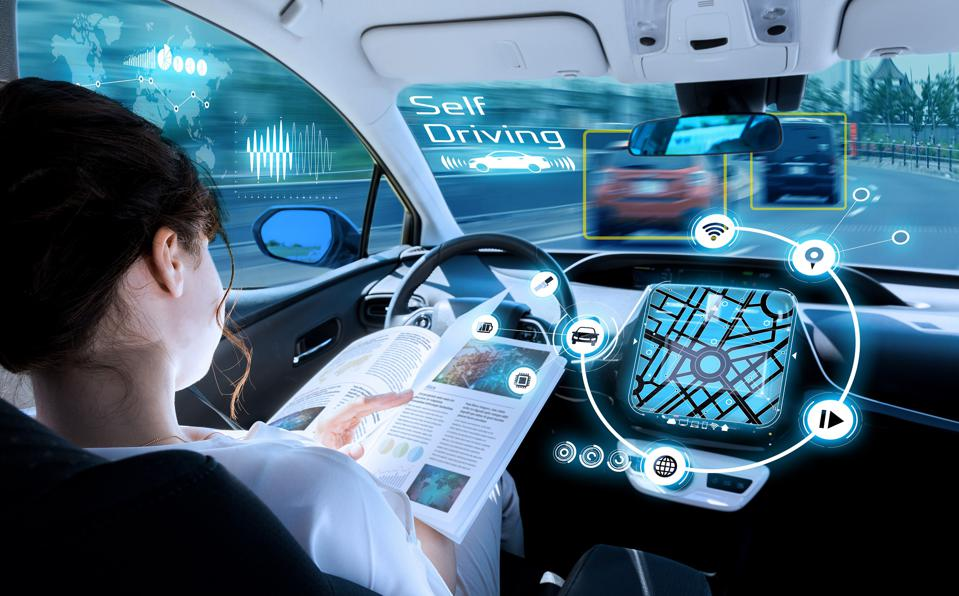
\includegraphics[width=5cm]{pics/Woman reading.png}
    \end{textblock*}
    \begin{itemize}
        \item Autonomous driving has a growing interest
              \begin{itemize}
                  \item More self-driving cars
                  \item Less human control
              \end{itemize}
        \item Pedestrians are the potential victims
              \begin{itemize}
                  \item Exposed to traffic dangers
                  \item No protection
              \end{itemize}
        \item Smartphones
              \begin{itemize}
                  \item Share location
                  \item Increase safety
              \end{itemize}
        \item Huge amount of data
              \begin{itemize}
                  \item 5G networks
              \end{itemize}
    \end{itemize}
\end{frame}

%------------------------------------------------
\section{State of the art}
%------------------------------------------------

\begin{frame}
    \frametitle{State of the art -- Communication}
    \begin{itemize}
        \item V2X -- Vehicle to everything
            \begin{itemize}
                \item Direct communication within short distances ($\sim$1km)
                \item WiFi technology in the licenced 5,9 GHz bandwidth
            \end{itemize}
        \item C-V2X -- Cellular vehicle to everything
            \begin{itemize}
                \item Prerequisite: Long-Term Evolution (LTE)
                \item Two operational modes:
                    \begin{itemize}
                        \item Direct communication over PC5 interface
                        \item Indirect communication over Uu-interface
                    \end{itemize}
                \item Long distance, latency-tolerant warnings
                \item Problem: LTE not fast enough for life-critical systems
            \end{itemize}
        \item C-V2X over 5G mobile-network
            \begin{itemize}
                \item Designed to deliver peak data rates up to 20 Gbps
                \item Beamforming technology
            \end{itemize}
    \end{itemize}
\end{frame}

\begin{frame}
    \frametitle{State of the art -- Prediction \& Scoring}
    \begin{itemize}
        \item There were several attempts in this area
            \begin{itemize}
                \item neural networks, decision trees and clustering algorithms
                \item Prediction time concidered to be optimal: $>$0,5s and $<$2s  
            \end{itemize}
        \item Most accurate former attempt
            \begin{itemize}
                \item Based on Mixed Markov-Chain Model (MMM)
                \item Accuracy score: 97\% with average delay of 783 ms
                \item With a new protocol via 5G this time can be reduced
				\item Reaction time: 500 ms (new developments are about to reach 10 ms)
            \end{itemize}
    \end{itemize}
    \begin{table}
        \begin{tabular}{l l l}
            \toprule
            \textbf{speed($\frac{km}{h}$)} & \textbf{speed($\frac{m}{s}$)} & \textbf{distance(m)} \\
            \midrule
                \;\;\;\;30         & \;\;\;8,3           & \;\;\;\;6,5             \\
                \;\;\;\;50         & \;\;13,8            & \;\;\;10,8              \\
                \;\;\;\;70         & \;\;19,4            & \;\;\;15,2              \\
                \;\;\;\;90         & \;\;\;25            & \;\;\;19,6              \\
            \bottomrule
        \end{tabular}
        \caption{Distance traveled during delay time}
    \end{table}
\end{frame}

%------------------------------------------------
\section{The Archangel protocol}
%------------------------------------------------

\begin{frame}
    \frametitle{The Archangel protocol -- Intro}
    \begin{itemize}
        \item P2V -- Pedestrian to Vehicle
        \item Prerequisites:
            \begin{itemize}
                \item 5G coverage
                \item Smartphone with 5G and Archangel-protocol capability
            \end{itemize}
        \item High reliability and fault tolerance
        \item Prediction, Scoring system, Warning messages
        \item Handles the case of street corners with thick walls 
    \end{itemize}
    \begin{figure}[h]
        \centerline{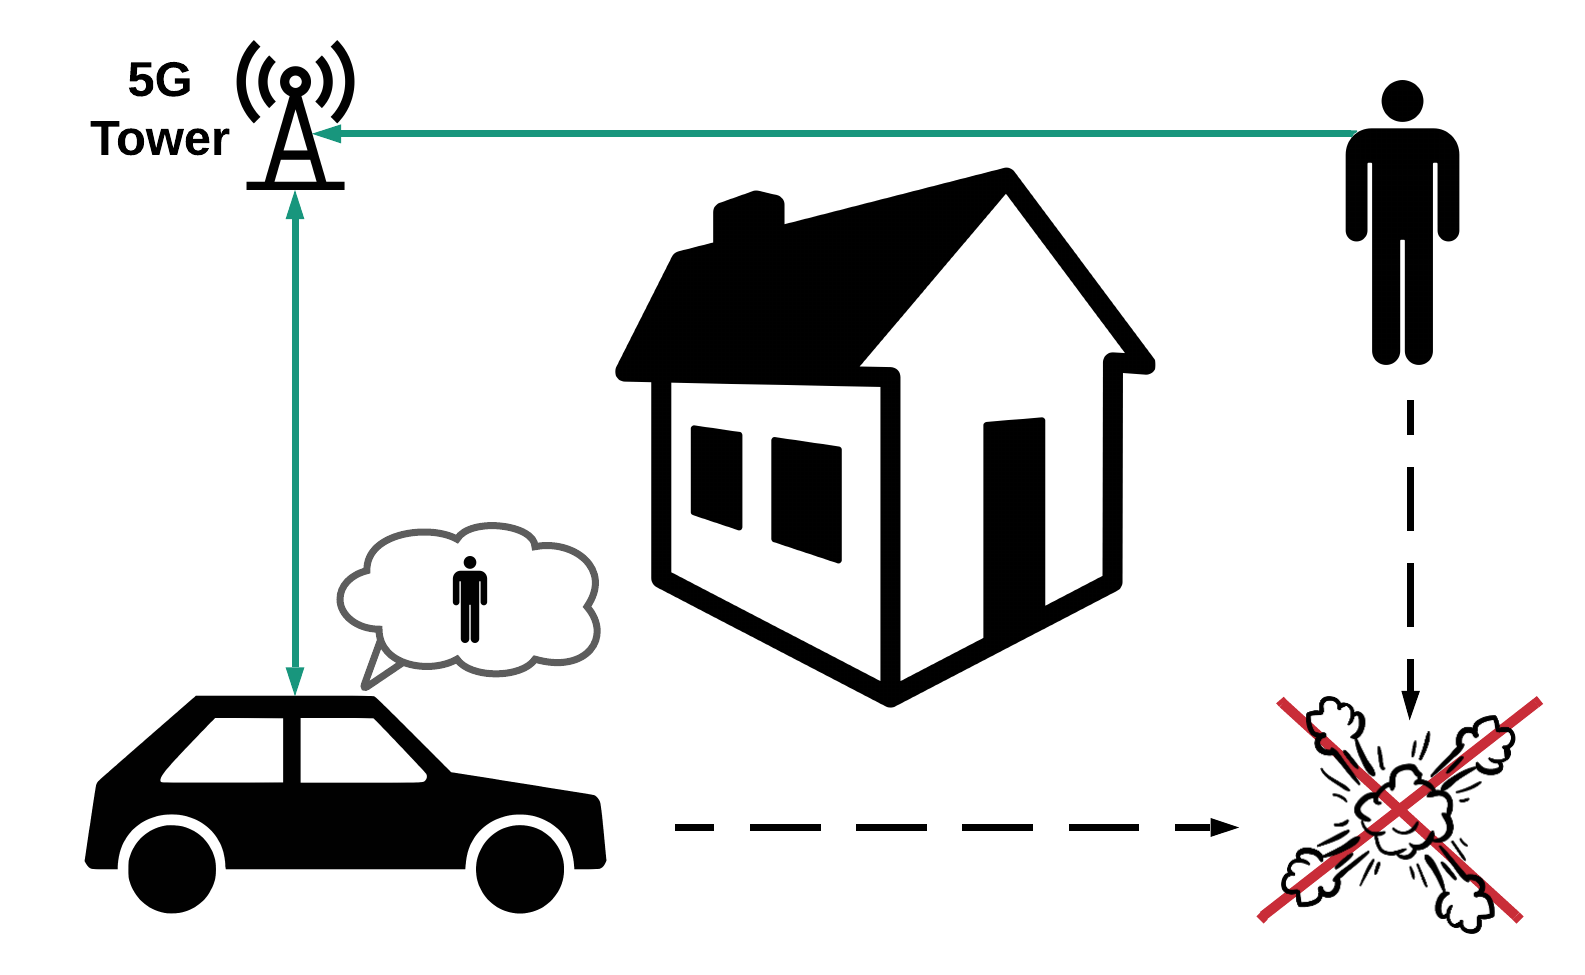
\includegraphics[width=4cm]{./pics/Corner.png}}
        \caption{Direct signaling blocked by a building}
        \label{fig}
        \end{figure}
\end{frame}

%------------------------------------------------
\subsection{Computational units}
%------------------------------------------------

\begin{frame}
    \frametitle{Computational units}
    \begin{textblock*}{5cm}(6cm, 0cm) % {block width} (coords)
        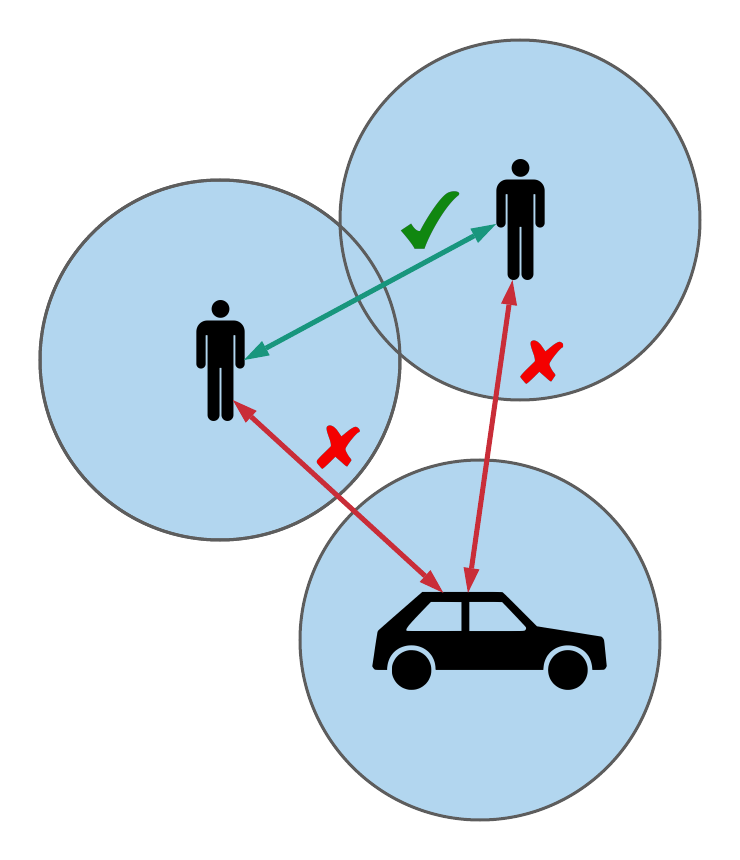
\includegraphics[width=5cm]{pics/Range of direct communication.png}
    \end{textblock*}
    \begin{itemize}
        \item Endpoints cannot process \\ large amount of data
        \item Border coverage is needed
        \item Centralized points
        \item High computing capacity
        \item Computations within \\ critical time constraints
        \item Precision
    \end{itemize}
\end{frame}

%------------------------------------------------
\subsection{Communication}
%------------------------------------------------

\begin{frame}[t]
    \frametitle{Communication}
    \begin{textblock*}{5cm}(2cm, 1.6cm) % {block width} (coords)
        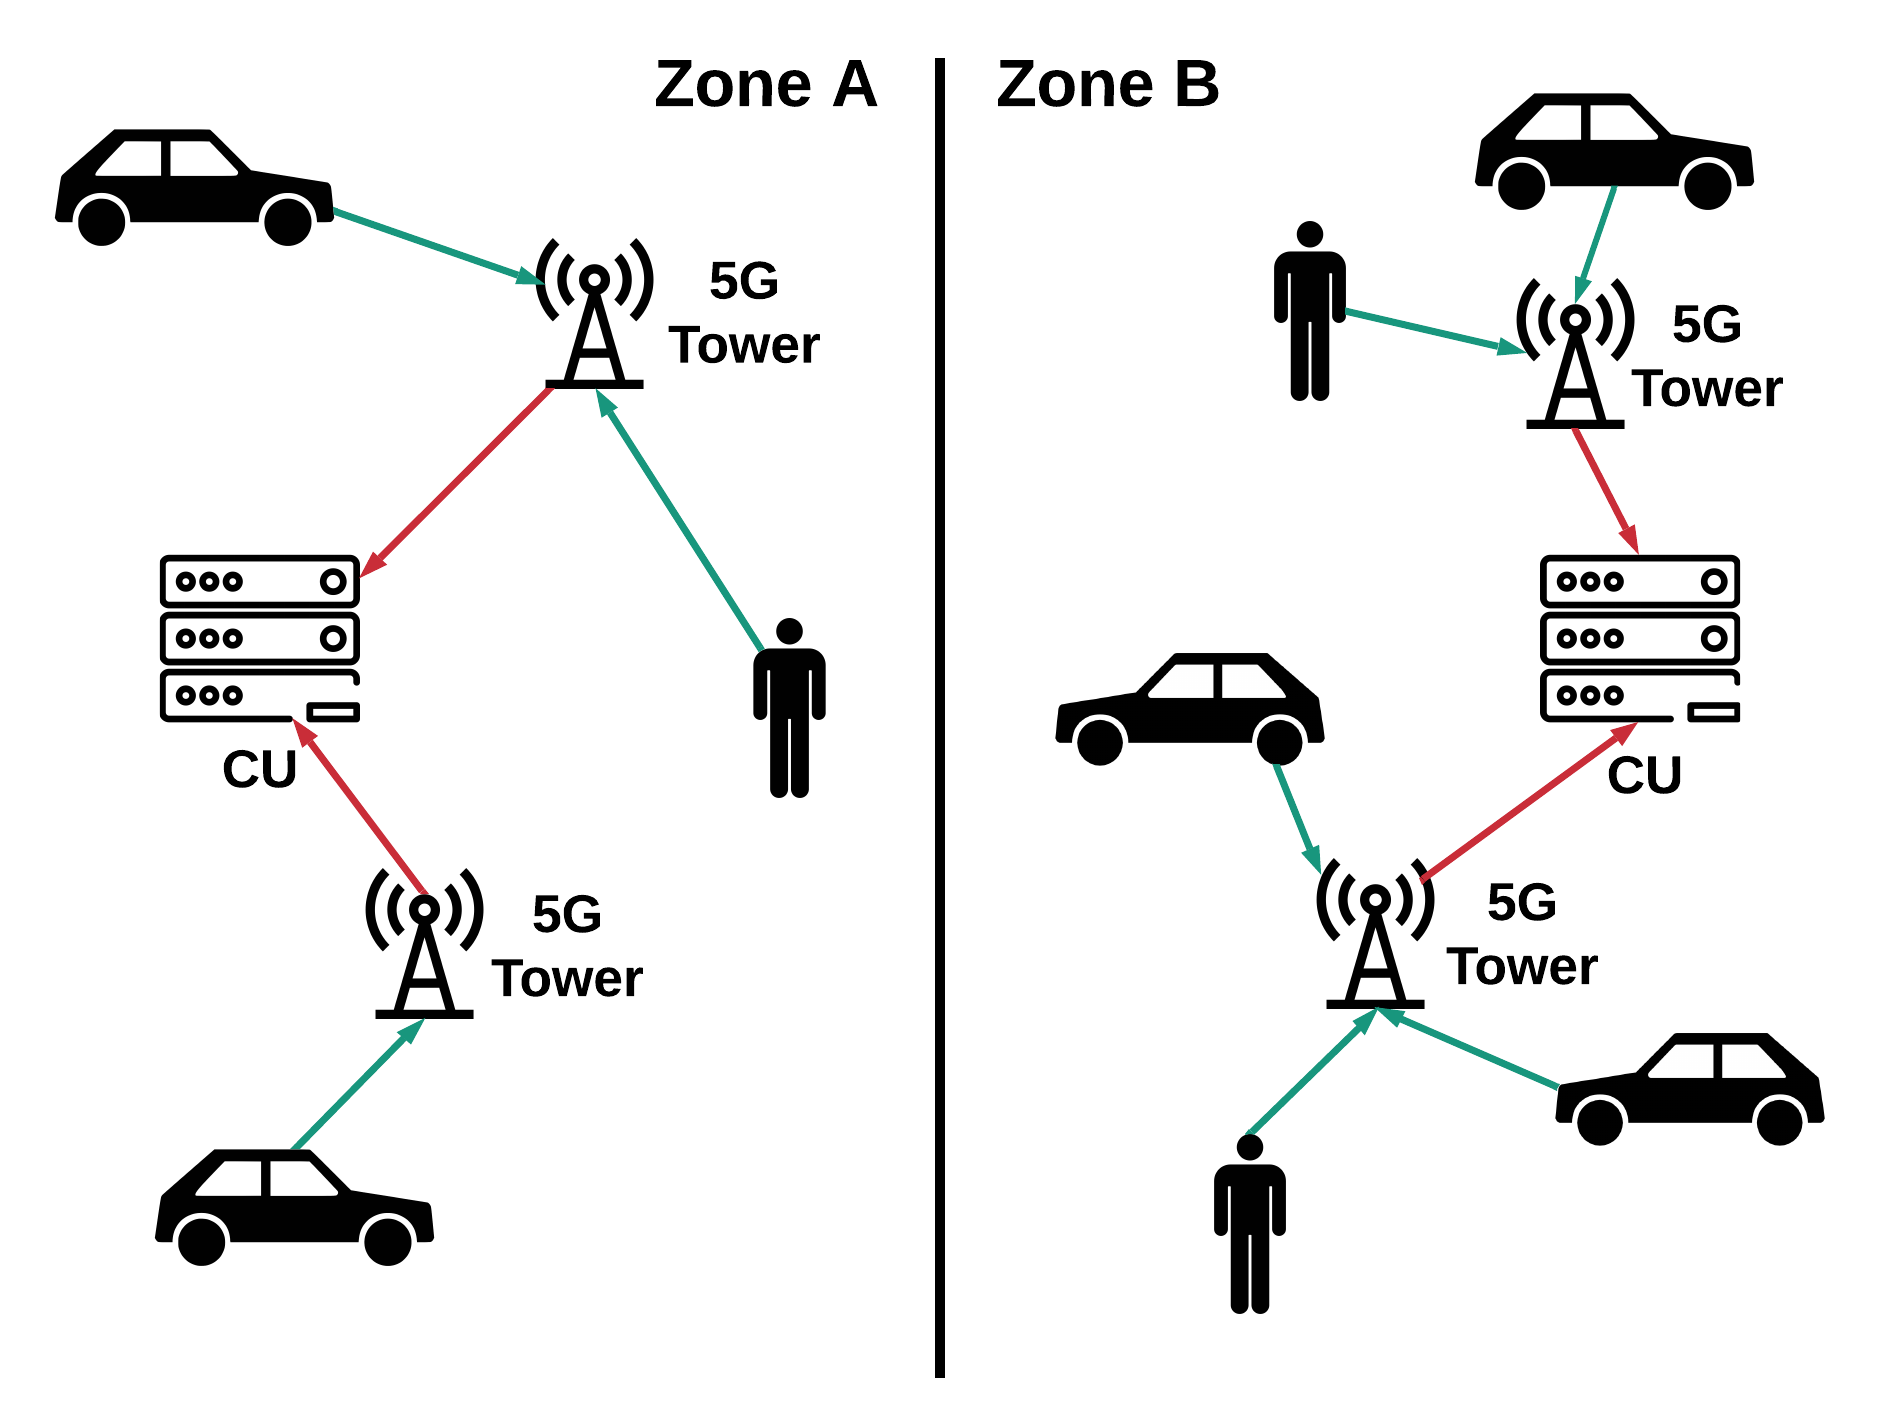
\includegraphics[width=8cm]{pics/Communication.png}
    \end{textblock*}
    \begin{itemize}
        \item Node $\rightarrow$ 5G Tower $\rightarrow$ Computational unit
        \item Area described by a given computational unit is a zone
    \end{itemize}
\end{frame}

%------------------------------------------------
\subsection{Edge case}
%------------------------------------------------

\begin{frame}[t]
    \frametitle{Edge case}
    \begin{textblock*}{5cm}(2cm, 3.3cm) % {block width} (coords)
        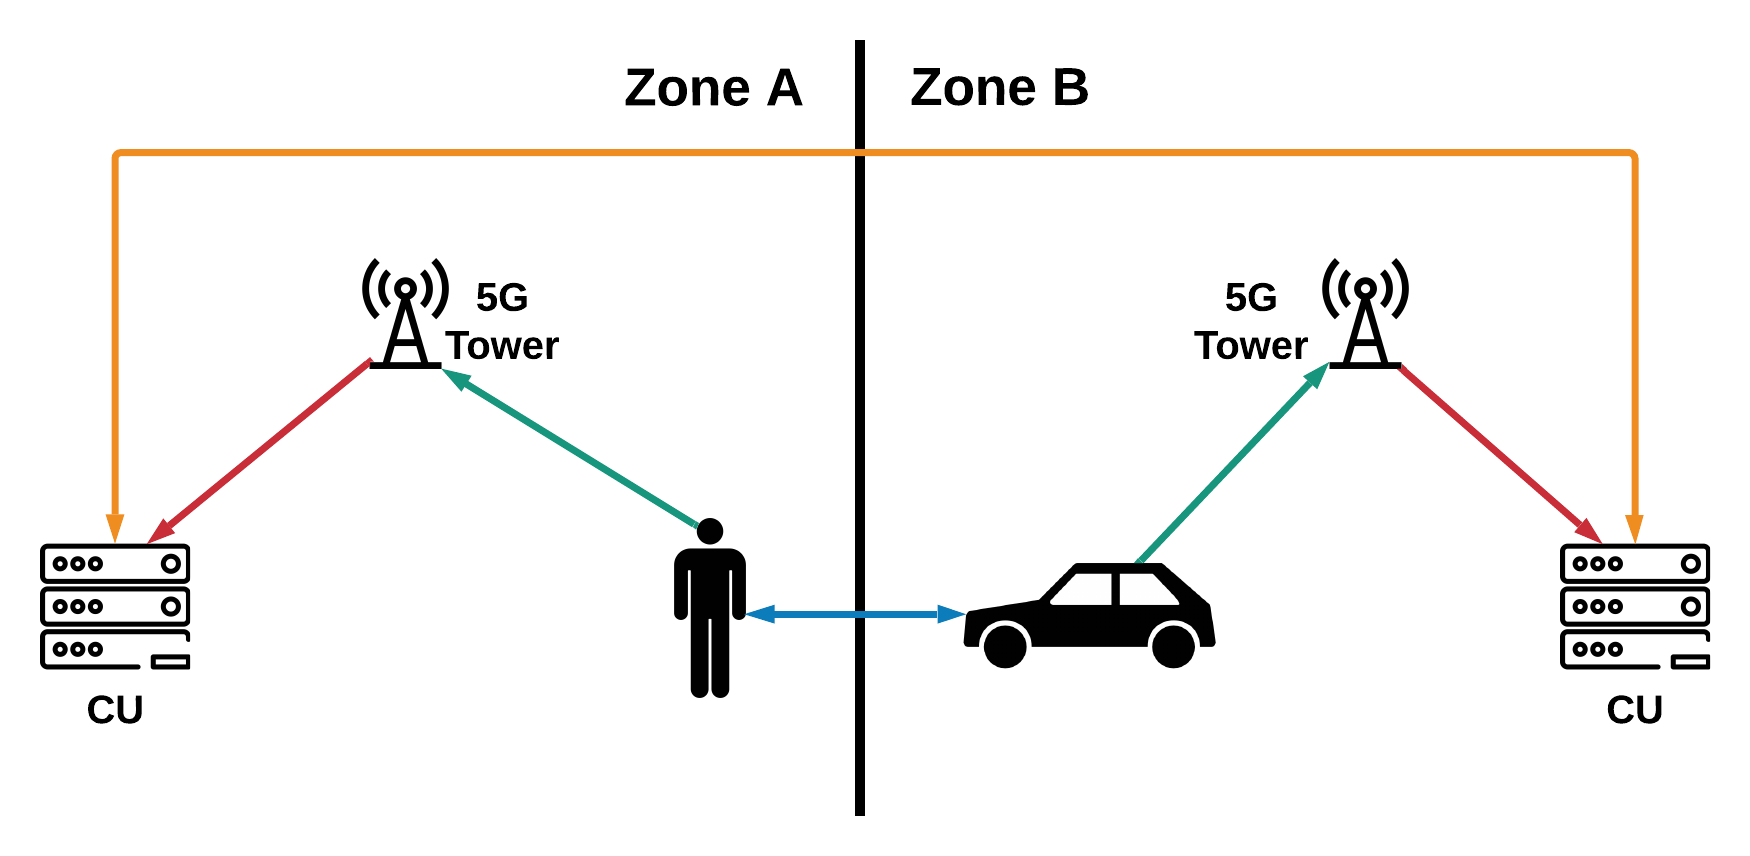
\includegraphics[width=8cm]{pics/Edge case.png}
    \end{textblock*}
    \begin{itemize}
        \item Pedestrian and a car in a separate computational zone
        \item The car’s computational unit needs to know the pedestrian’s data
        \item Which of the two CUs should calculate the data for the car?
              \begin{enumerate}
                  \item Optimal case $\rightarrow$ The CU which is in the zone of the car
                  \item Network round trip to save time in case when \\ the car's CU is already critically loaded
              \end{enumerate}
    \end{itemize}
\end{frame}

%------------------------------------------------
\subsection{Scoring system}
%------------------------------------------------

\begin{frame}
    \frametitle{Scoring system}

    \begin{itemize}
        \item Analysis of the situation
        \item Define the order of urgency between the notifications
    \end{itemize}
    \begin{columns}
        \begin{column}{0.5\textwidth}
            \begin{block}{Calculations - key points}
                \begin{itemize}
                    \item movement
                    \begin{itemize}
                        \item speed
                        \item direction
                    \end{itemize}
                    \item position
                \end{itemize}
            \end{block}
        \end{column}
        \begin{column}{0.4\textwidth}
            \begin{figure}
                \centering
                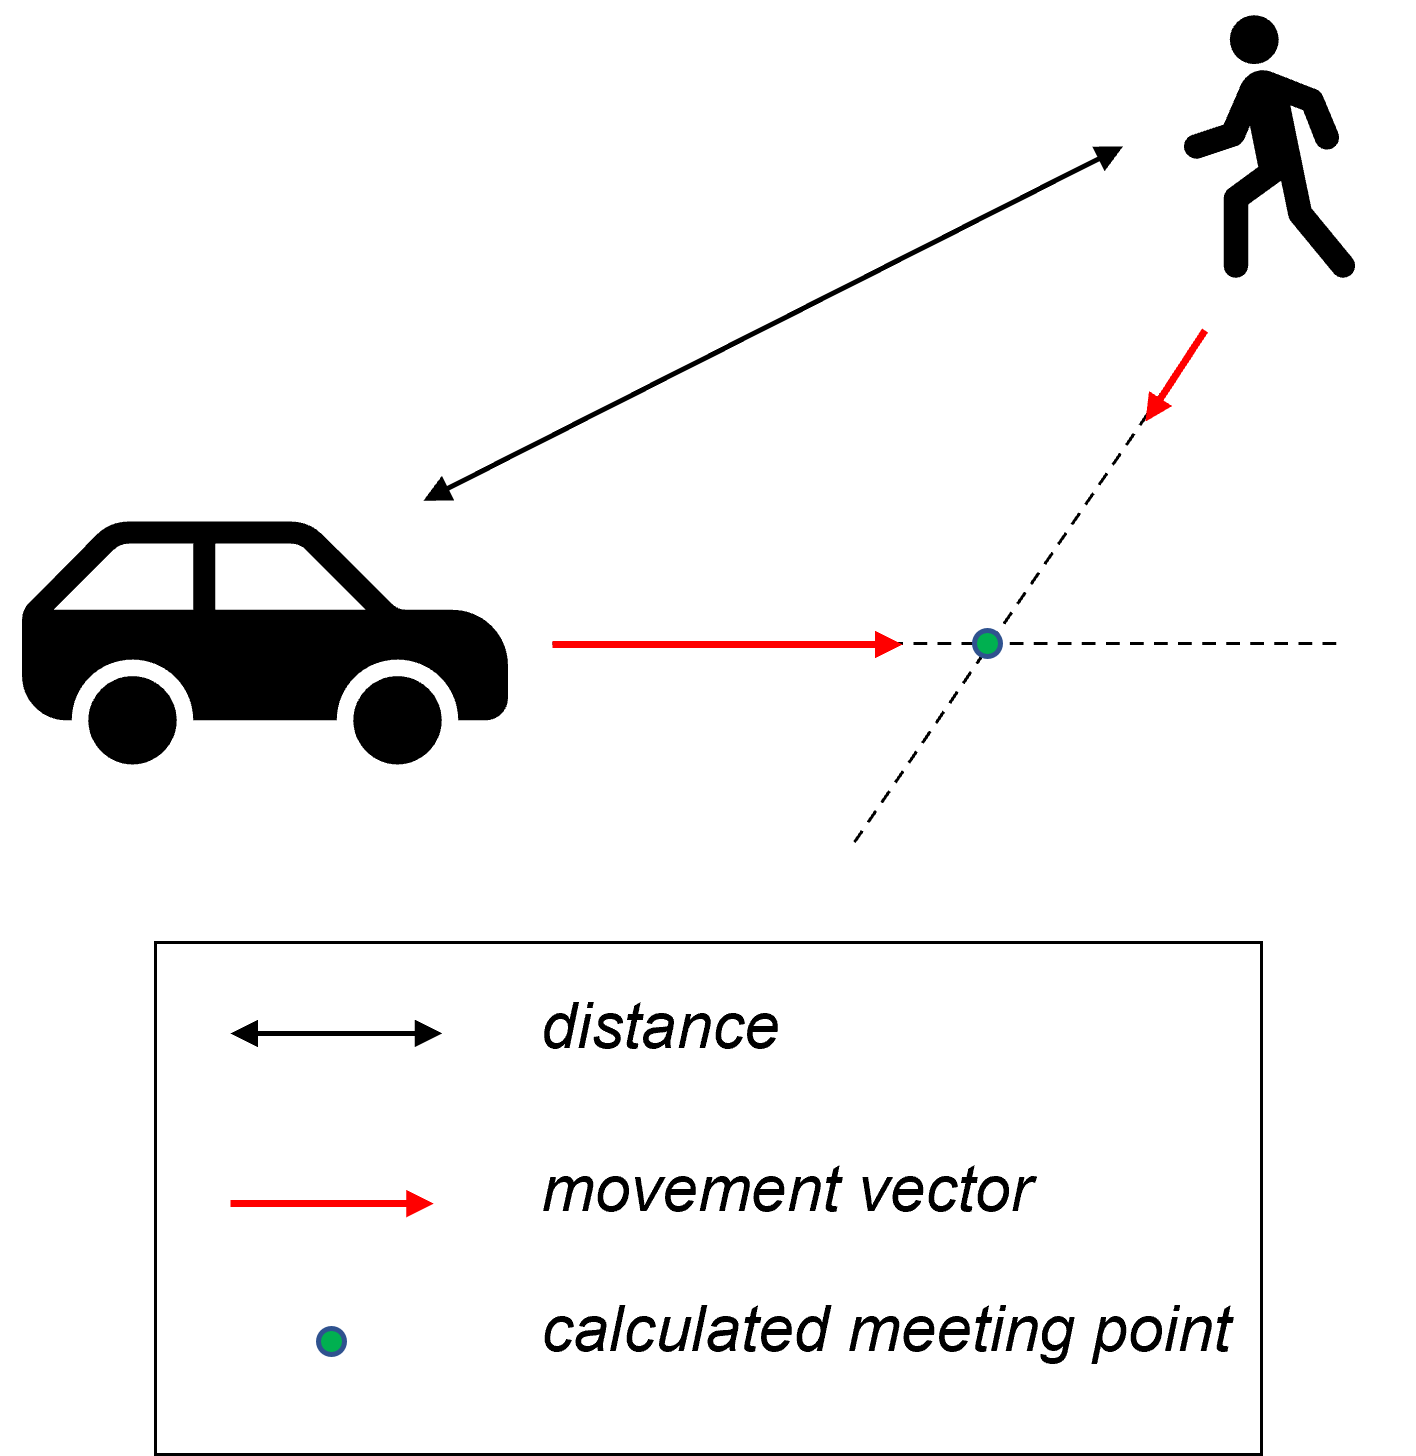
\includegraphics[width=1\textwidth]{pics/Core factors of the calculation}
            \end{figure}
        \end{column}
    \end{columns}
\end{frame}

\begin{frame}{Scoring system}
        \begin{block}{Environment}
            If data is available about the environment, it can increase or decrease the score.
        \end{block}
        \vspace{0.1cm}
        \centering
        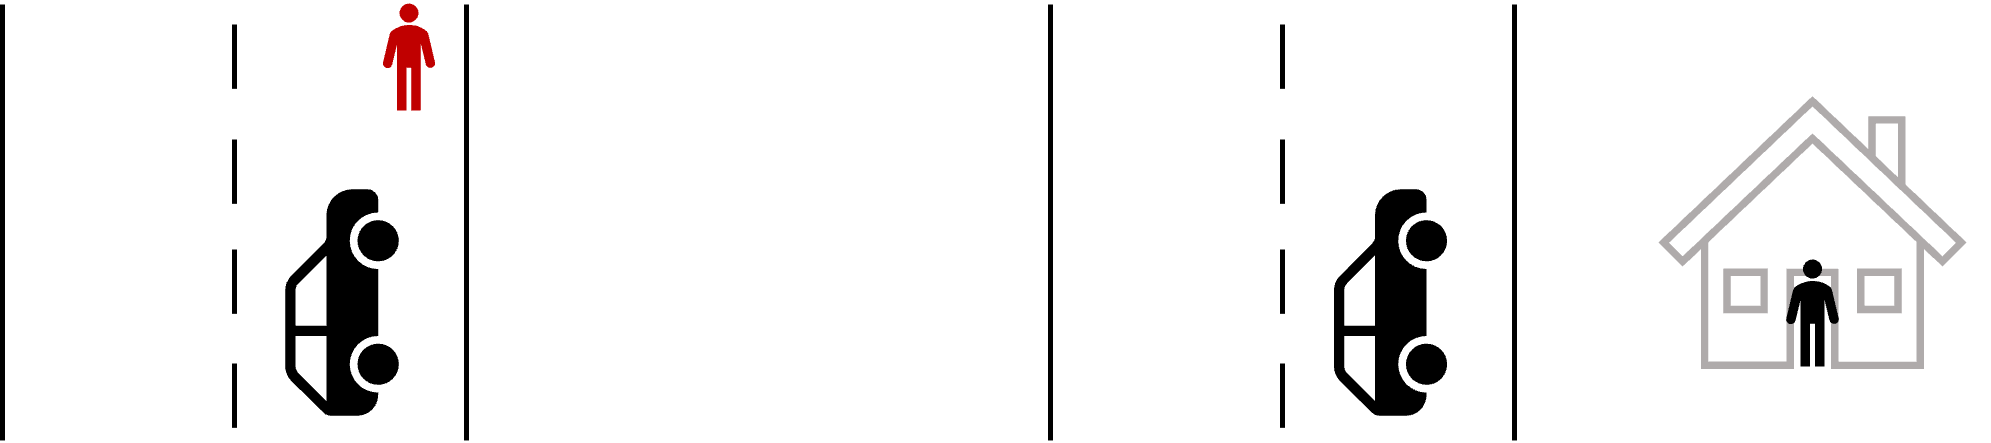
\includegraphics[width=0.6\textwidth]{pics/environment}
        \vspace{0.5cm}
        \begin{block}{Predictions}
            The last part of the score calculation is to assess the possibility of certain routes and to predict movements.
        \end{block}
        \centering
        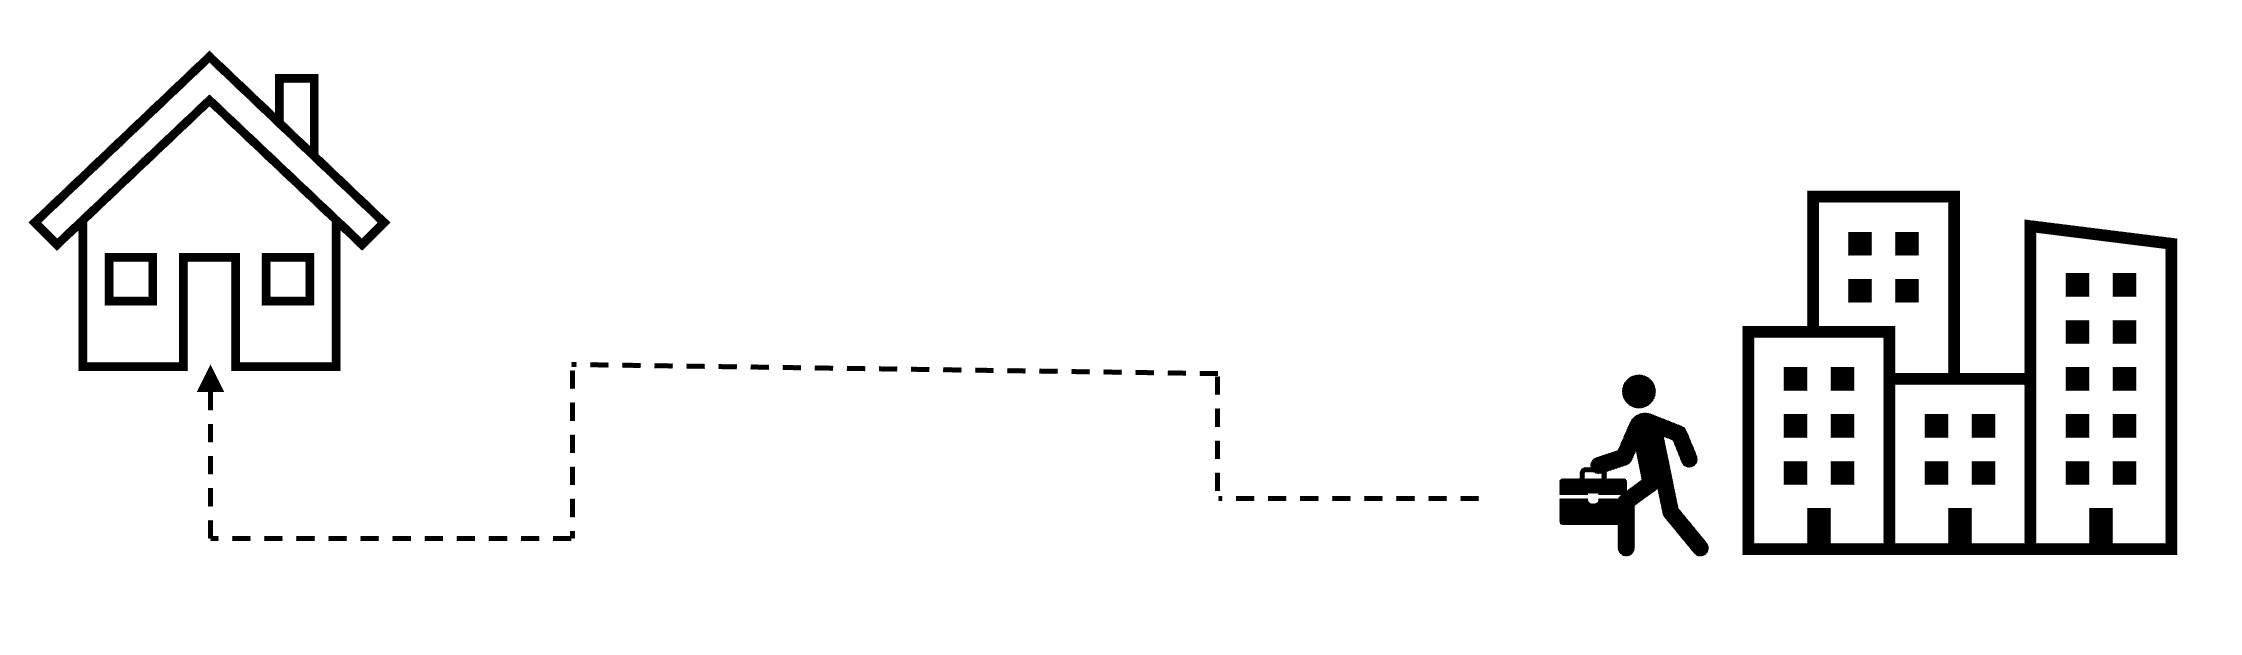
\includegraphics[width=0.6\textwidth]{pics/route_prediction}

\end{frame}

%------------------------------------------------
\subsection{Package structure}
%------------------------------------------------

\begin{frame}
    \frametitle{Package structure}
    \begin{textblock*}{5cm}(2cm, 3.3cm) % {block width} (coords)
        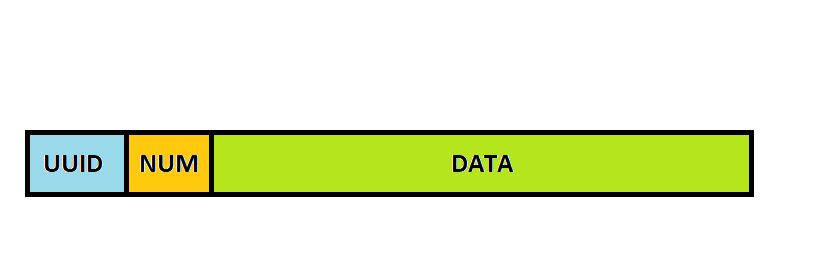
\includegraphics[width=8cm]{pics/Package structure.png}
    \end{textblock*}
    \begin{itemize}
        \item UUID
            \begin{itemize}
                \item Number of UUIDs
                \item For example:  123e4567-e89b-12d3-a456-426614174000
            \end{itemize}
        \item Serial number
        \item Data type code
        \item Actual data
            \begin{itemize}
                \item Coded
                \item Compressed
            \end{itemize}
    \end{itemize}
\end{frame}

%------------------------------------------------
\section{Conclusion}
%------------------------------------------------

\begin{frame}
    \frametitle{Conclusion}
    \begin{itemize}
        \item Future = self-driving cars
        \item Our work
        \item Future plans
    \end{itemize}
\end{frame}

%------------------------------------------------

% \begin{frame}[fragile] % Need to use the fragile option when verbatim is used in the slide
%     \frametitle{Verbatim}
%     \begin{example}[Theorem Slide Code]
%         \begin{verbatim}
% \begin{frame}
% \frametitle{Theorem}
% \begin{theorem}[Mass--energy equivalence]
% $E = mc^2$
% \end{theorem}
% \end{frame}\end{verbatim}
%     \end{example}
% \end{frame}

%------------------------------------------------

% \begin{frame}
%     \frametitle{Figure}
%     Uncomment the code on this slide to include your own image from the same directory as the template .TeX file.
%     %\begin{figure}
%     %\includegraphics[width=0.8\linewidth]{test}
%     %\end{figure}
% \end{frame}

%------------------------------------------------

% \begin{frame}[fragile] % Need to use the fragile option when verbatim is used in the slide
%     \frametitle{Citation}
%     An example of the \verb|\cite| command to cite within the presentation:\\~

%     This statement requires citation \cite{p1}.
% \end{frame}

%------------------------------------------------

% \begin{frame}
%     \frametitle{References}
%     \footnotesize{
%         \begin{thebibliography}{99} % Beamer does not support BibTeX so references must be inserted manually as below
%             \bibitem[Smith, 2012]{p1} John Smith (2012)
%             \newblock Title of the publication
%             \newblock \emph{Journal Name} 12(3), 45 -- 678.
%         \end{thebibliography}
%     }
% \end{frame}

%------------------------------------------------

\begin{frame}
    \Huge{\centerline{The End}}
\end{frame}

%----------------------------------------------------------------------------------------

\end{document}